\documentclass[b5j,12pt]{jsbook}
%\documentclass[b5j,10pt,tombo]{jsbook}

%\pagestyle{plain}

\usepackage[dvipdfmx]{graphicx}

% フォントメトリック指定
\usepackage{minijs}
\usepackage{otf}

\usepackage{makeidx}
\usepackage{booktabs}
\usepackage{tabularx}
\usepackage{wrapfig}
\usepackage{moreverb}
\usepackage{amsmath}
\usepackage{amssymb}
\usepackage{fancybox}
\usepackage{ascmac}
\usepackage{listings,jlisting}
\usepackage[avantgarde]{quotchap}

%\renewcommand{\baselinestretch}{0.5}
%\renewcommand{\baselinestretch}{0.6}
\renewcommand{\baselinestretch}{1.0}


\begin{document}
\title{ゆるいSQL}
\author{AliceSystem インフラエンジニアの毒舌な妹 ありす ゆう 共著}
\date{初版発行 2019年4月14日}
\maketitle
\frontmatter
\section*{謝辞}
\begin{center}
この本を読んでくださる方に \\
気力をくれる友人に \\
大切な人に \\
感謝と本書をささげます
\end{center}

\section*{前書き}





\section*{本書の内容}

\paragraph{第一章}

\paragraph{第二章}

\paragraph{第三章}

\paragraph{第四章}


\section*{免責事項}
本書に書いてあることは、筆者知識のレベルでまとめたものです。ですが、内容が正しいとは言い切れません。初版でも改訂版でも相当やらかしています。また、学校のレポート、業務などのコードを書く際に、本書の内容を信じて書いて損害が生じても、筆者にその責任はありません。

くれぐれも、自己責任と十分な検証の上、ご利用ください。

\section*{表紙イラスト}
ゆうちゃん (コース英知)
\tableofcontents
\listoffigures
\mainmatter

\chapter{SQLの本をどう選ぶ?}

SQLを学ぼうとするとき、はず、参考書を探すというのはよくあることです。ですが、署名にSQLとついた本を書店で眺めたり、Amazonあたりのネット通販で眺めたりしたとき、どの本を手に取っていいか分からなくなることがあります。

本書では、最初に、SQLを学ぶための本の選択の仕方について記載します。

\section{sQLの本とRDBMSの本は違う}

たとえば、AmazonでSQLをキーワードに和書を検索したら、どのくらいの本が出てくるのでしょうか。2019年3月現在で、和書、洋書、Kindoleを問わずに検索すると、1000種類以上の検索結果が出てきます。

この数では、SQLそのものを学ぶために、どの本を手に取ったらいいか分からなくなります。署名だけで買ってみると、SQLについては全くあっ枯れていない本を引き当ててしまうこともあります。

なぜこのような混迷したことになっているか、というと、SQLという単語が署名につく本には、データベースを操作する言語としてのSQLそのものについて書いてある本と、操作にSQLを使うことができる、リレーショナルデータベース実装の取り扱いについての本と、両方が含まれるためです。

このような混乱を招くのは、SQLを使用することができるリレーショナルデータベースの実装で、書籍が出るくらいメジャーなものは、なんとかSQL,もしくはSQLなんとか、という名前がついていることです。単独で書籍が出るものだと、Microsoftの製品のSQL-Serverや、Oracleに吸収されたMySQL ABのMySQL、PostgreSQLがあります。また、PHPなどに組み込まれている、ソフトウェア組み込み用のデータベースのSQL-Liteというものもあります。

もちろん、なんとかSQLでないリレーショナルデータベースもあります。有名なところでは、Oracle,DB2といった商用データベース、オープンソースだと、FireBirdや、MySQLからフォークした、MariaDBなどがあります。

\subsection{SQLの本}

書名で、SQLの前にも後にもなんとかと付かない本は、SQLそのものについて記述した本になります。たとえば、はじめてのSQL、SQL入門、というタイトルの本は、間違いなく、SQLそのものについて、考え方や書き方の説明をしている本です。

ここでいう、SQLそのものとは、たとえば、SELECTによる検索、CREATEによるテーブルの生成、UPDATEやDELETEによるれこーどのそうさなどについて書いてある本ということです。つまり、SQLという言語の解説書は、おおむね、SQLの前後になんとかとつかない署名を採用しています。

とはいえ、当然ながら、例外というものがあります。それは、特定データベース製品のためにSQLを拡張した言語の入門書は、なんとかSQL、という名前で、その拡張した言語を説明することがあります。

この例として、Oracleが、データベースの自社製品であるOracleのためにSQLを拡張した言語、PL/SQLの解説書が挙げられます。PL/SQLという言語の入門書は、当然、PL/SQLという言語名を、署名に織り込んでいます。

同じように、Microsoftのデータベース製品、SQL-ServerのためにSQLを拡張した言語、Transaction SQL(T-SQL)を解説する本は、T-SQLという言語名から署名を取っているでしょう。そのほかにも、Salesforceが自社SaaSデータベースの操作のためにSQLを拡張した言語は、SOQLという名前です。この言語の解説書が出るときは、SOQLという言語名が署名に付くこととなります。、


\subsection{RDBMSの本}

署名に、リレーショナルデータベースのプロダクトの名前が付いている本は、おおよそ、そのデータベースのインストールや運用、管理、バックアップ取得、などオペレーションの入門書となります。

MySQL入門、PostgreSQL入門、というような署名は、MySQLやPostgreSQLといった、データベースプロダクトのオペレーションについて解説した本です。メンテナンスに必要なコマンドとしてSQLについてこうをさいていることはありますが、SQLについて詳細な説明はありません。

これらの本は、データベースをインストールしたり運用したりする、サーバエンジニアやデータベースアドミニストレータに向けた本です。そのため、SQLを学ぼうという人のための本とは、役割が異なります。


\section{どんなSQLの本を選べばいいのか}

では、言語としてのSQLを学ぼうというときに、どのようなSQLの本を選択すればよいのでしょうか。筆者の個人的な見解を交えつっつ、簡単にまとめてみます。

大型書店では、立ち読み用のコーナを切歯していることが増えました。ですが、そこで、置いてある本の内容をすべて読破するわけにもいきません。どのようなところに、注目すればよいのでしょうか。

\subsection{よさそうな入門書を判断するポイント}

筆者がSQLの入門書を選ぶと木、どのようなところを見るかを節瞑します。ただし、これは筆者の見解であり、特定の書籍を持ち上げ、またはおとしめるものではありません。

SQLの入門書を判断するポイントは、テーブルとレコード、アトリビュートという概念を、どう説明しているかだと、筆者は考えています。

多くの入門書では、テーブルは表計算ソフトの表のようなもの、レコードが行でアトリビュートが列、というような説明をされていることが多いです。筆者の見解として、このような説明をしている入門書は、あまりおすすめしません。
テーブルが表であるというイメージが付いてしまうと、複雑なクエリを書いたりするときに、レコードとレコードの関係がうまくイメージができない、というのが筆者の見解です。

では、どのような説明をしている本がよいのでしょうか。それは、テーブルを丸でかこった空間で表し、レコードをその中のどこかにあるものとして表現している本です。テーブルとレコードを、このような表し方をしている本だと、おすすめできます。

\begin{figure}[htbp]
	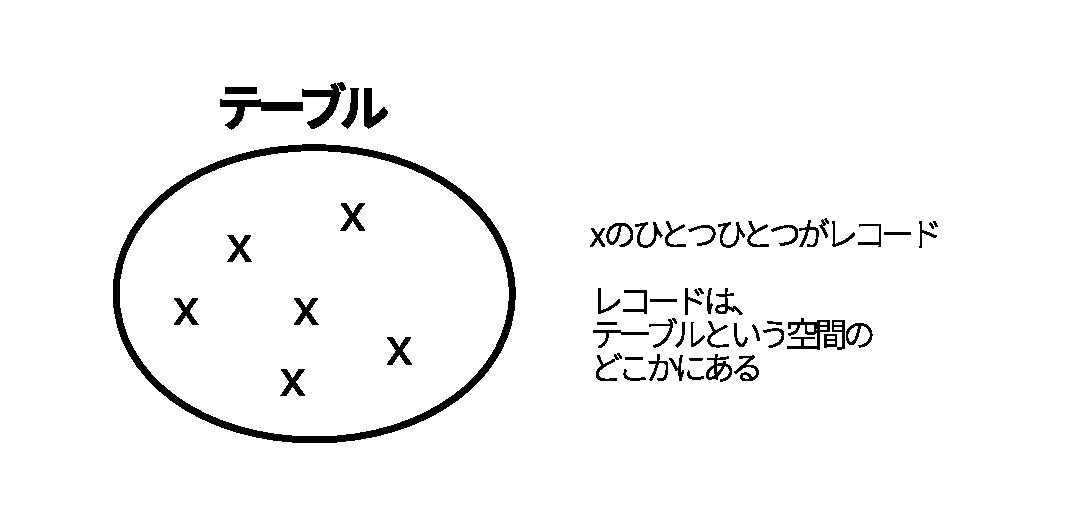
\includegraphics[width=12cm,clip]{draw/table.eps}
	\caption{テーブルとレコード}
	\label{fig:animals_kinds_er}
\end{figure}



\subsection{SQLをより深く学ぶために}

SQLが何をやっているのかをより深く理解したくなったときは、数学の集合論と命題論理を学ぶことをおすすめします。

SQLのテーブルは、集合論でいうところの集合に相当します。そして、SELECTという操作は、命題論理で言うところの命題であり、集合論的な見地での関数に相当します。

本書では数学的な厳密さには立ち入りませんが、必要となったときは、集合論の扉を開いてみる、ということを覚えておいていただければと思います。


\chapter{テーブルとレコードとアトリビュート}

SQLを学ぶために、まず、テーブルとレコードとアトリビュートは、どのようなものかを見ていくことにしましょう。前の章で、テーブルは丸、レコードはその丸の中のどこかにあるもの、という説明をしました。そして、アトリビューtについての説明ははしょりました。ぎt

この章では、この先SQLを学ぶのに必要なこととして、テーブルとレコードとアトリビュートについて、学び直していくことにします。


\section{テーブル}

リレーショナルデータベースのテーブルとは、どのようなものでしょうか。一言で言ってしまえば、レコードという要素がどこかに存在する空間です。レコードは、この空間の中のどこかにある要素となります。

\subsection{テーブルの中でレコードはどこにあるのか}

テーブルの中で、レコードはどこにあるのでしょうか。テーブルという空間の中で、レコードがどこにあるかは、そのレコードのアトリビュートの値で決まります。詳細は後で説明しますが、アトリビュートが座標と考えることができます。

たとえば、整数のアトリビュートを一つだけ持つレコードが定義されているとします。このとき、レコードを、数直線上のその値に対応している馬謖尾置いたと考えます。そうすると、テーブルという空間は数直線の形をしていて、レコードの場所は、その数直線上のどこかという様に考えることができます。


\subsection{テーブルの中身には順番がない}


テーブルの中にはレコードがあるわ出ですが、そのレコードにはなんらかの順番があるのでしょうか。結論から行けば、テーブルの中にあるレコードに、順番はありません。データベースに登録した順番や、特定のアトリビュートの値が順番になるのではありません。データベースのなかでは、レコードは順番が定義されません。

大切なことなのでもう一度言いますが、テーブルの中のレコードには、順番がありません。これは、読み出しを行ったとき、入れた順番や、プライマリキーの値の順番で結果が取り出せることを期待してはならない、ということです。
これは、limitを使ってひとつだけ要素を取り出す場合、特定のレコードが必ず取り出せることを期待s知恵はならないということでもあります。


では、ORDER BYで定義される順番はなんなのでしょうか。それは、データベースから取り出すときにソーティングを行って、定義された順番で並べています。そのため、順番で取り出す必要が無いときは、ORDER BYを書かない方が読み出しは早くなります。

\subsection{普通の麻雀と鷲巣麻雀}



\subsection{順番はどうやってつけるのか}

\section{レコードとアトリビュート}


\subsection{アトリビュートの役割と座標軸}

\subsection{テーブルという空間}

\subsection{多次元空間}
\chapter{SELECTするってどんなこと}


\section{SELECTの性質}

\subsection{元のテーブルは変化しない}

\section{SELECTとテーブル}
%\chapter{SQLと関数、あるいはもう制御構造なんかいらない}
\chapter{NULLと三値論理}

SQLで用いられる値には、NULLというものがあります。では、NULLはどのような意味を持つのでしょうか。また、NULLを判定に使うというのは、どのようなことなのでしょうか。

この章では、少しばかりわかりにくいNULLのはなしをします。

\section{SQLとNULL}

リレーショナルデータベースのテーブルのアトリビュートとして、NULLというものがあります。このNULLは、あるレコードのアトリビュートに入れるべき値が無いときに使われるものです。

テーブルをCREATEするときに、アトリビュートにNOT NULL制約をつけて、NULLを許容しないようにすることができます。また、NULLは、リレーショナルデータベースで許容すべきか否か、という根本的な問題もあります。そんなNULLとは、どんな存在なのでしょうか。

たとえば、二つのアトリビュートをもつテーブルがあり、あるレコードについては、その一つしか値が決まらなかったとします。そのレコードについて、もうひとつの、値が決まっていないアトリビュートに入っている値がNULLです。

その一方で、あるテーブルにおいて、全てのアトリビュートがNULLであるレコードは存在しません。レコードの情報がなにも無い、ということイコール、そんなレコードは存在しない、ということだからです。つまり、アトリビュートにNULLをとるレコードは、少なくともひとつのアトリビュートは、NULLでない値が入っていなければならないということになります。

コンピュータの言語では、変数などの値が設定されていない状態をさして、NULLである、という言い方をします。また、ポインタの値として、NULLで初期化し、積極的に未設定であることをアピールすることもあります。




\subsection{NULLの意味}

では、リレーショナルデータベースとSQLで、NULLはなにをあらわしているのでしょうか。NULLの意味はふたつあります。ひとつは、それについては知らないという情報を表す値であると言うことです。そして、もうひとつの意味は、それについて適用できるものが無い、という情報をあらわします。

では、NULLのふたつの意味は、どのように区別されるのでしょうか。

\subsubsection{知らないというNULL}

\begin{figure}[htbp]
	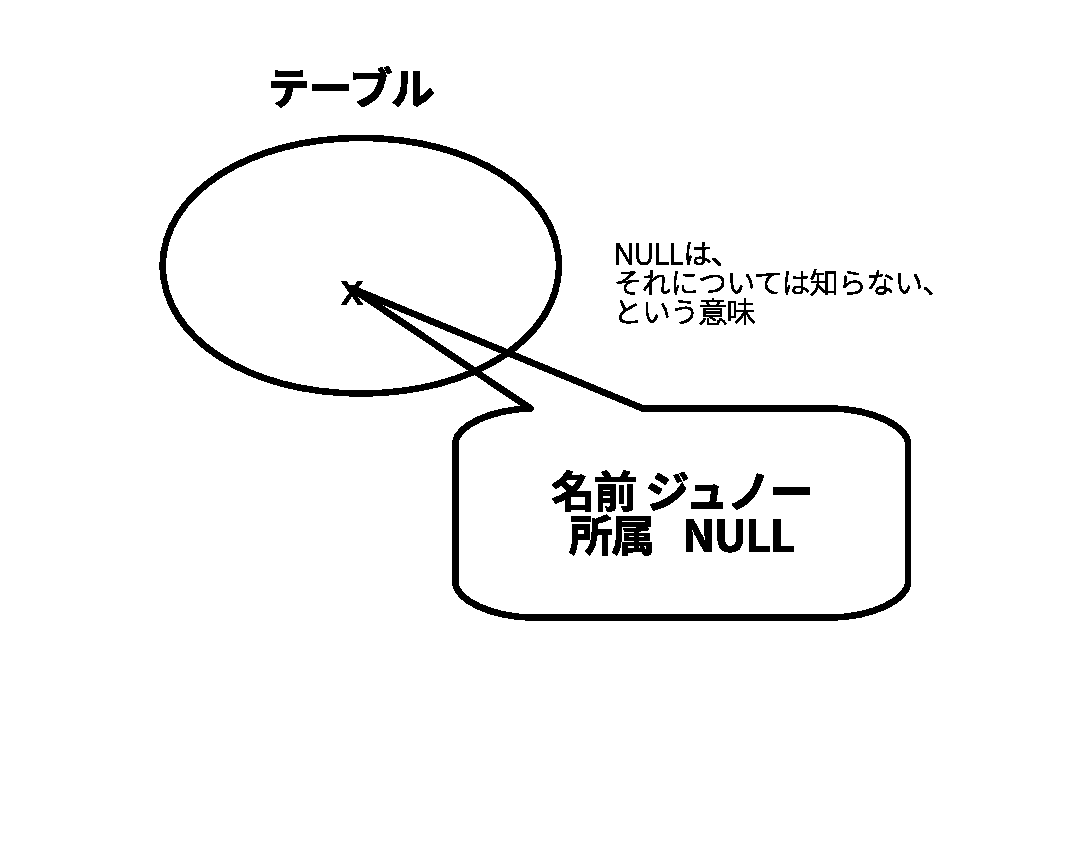
\includegraphics[width=12cm,clip]{draw/null.eps}
	\caption{NULLをもつレコード}
	\label{fig:record_with_null}
\end{figure}
たとえば、名前と所属という二つのアトリビュートをもつテーブルを考えます。あるレコードで、所属の値がNULLであれば、それは、所属が分からない、という意味になります。

また、レコードにINSERTするとき、アトリビュートの値としてNULLが設定されているということは、その値を決定する情報がない、ということです。このような場合、NULLとは、unknownである、知らないということであると解釈するのが自然です。

\subsubsection{適用できないというNULL}

animalsというテーブルは動物の名前と、動物の種別idをアトリビュートとして持っているとします。kindsテーブルは、idと、動物の種別名を持っています。つまり、kindsは動物の種別名マスターです。

この二つのテーブルは、図\ref{fig:animals_kinds_er}のような関係にあるとします。このとき、animalsに、kindsに種別名が入っていない動物の情報を入れたくなったときはどうしたらよいでしょうか。そのような登録を許さないという流儀もありますが、ここでは、そのような登録を許すことを前提に考えてみます。

動物の種別マスタであるkindsに鳥類の登録がないのですが、animalsにはペンギンを登録します。このとき、kindidはマスタ側にて基油できるものが無いため、NULLとします。

このようなケースでは、animalsのレコードで、アトリビュートkindis.animalsに、ますた側に適用できるものがない、という意味でNULLを入れます。

これは、LEFT JOINやRIGHT JOINといった、左右の外部結合で必要になる考え方です。左右の外部結合は、JOINの結果であるテーブルに、適用できるものがなかった、という意味のNULLを許容します。これについては、後の章で、あらためて説明します。

\begin{figure}[htbp]
	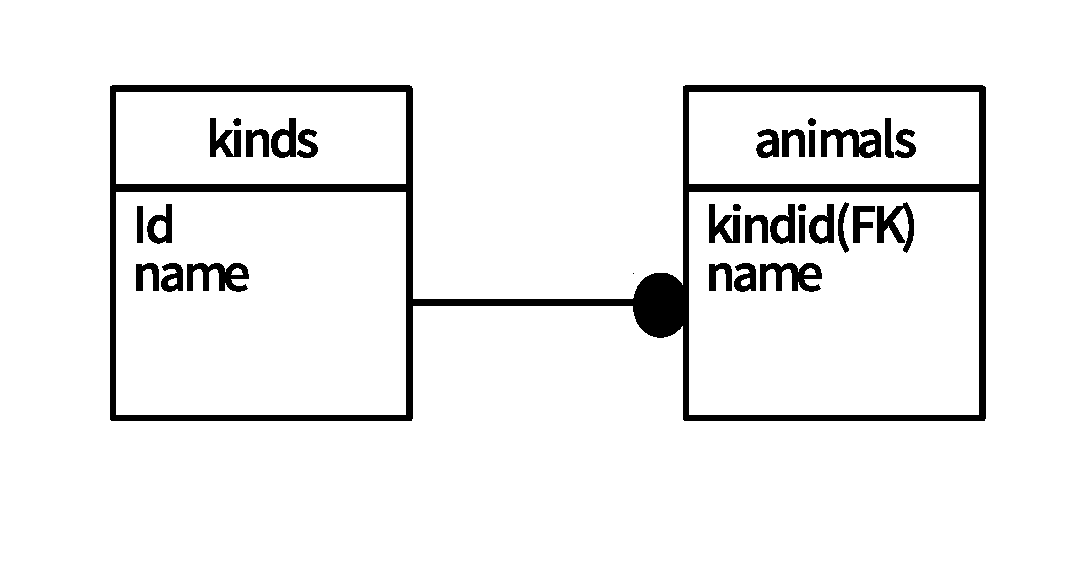
\includegraphics[width=12cm,clip]{draw/null_er.eps}
	\caption{animalsとkindsのER図}
	\label{fig:animals_kinds_er}
\end{figure}

\begin{table}[htb]
  \begin{tabular}{|c|c|} \hline
    id & name \\ \hline
    1 & 哺乳類 \\
    2 & 爬虫類 \\
    3 & 魚類 \\ \hline
  \end{tabular}
  \label{table:kinds}
  \caption{kindsテーブルの内容}
\end{table}

\begin{table}[htb]
  \begin{tabular}{|c|c|} \hline
    kindid & name \\ \hline
    1 & パンダ \\
    2 & 亀 \\
    3 & はまち \\
    NULL & ペンギン \\ \hline
  \end{tabular}
  \label{table:animals}
  \caption{animalsテーブルの内容}
\end{table}


\subsection{NULLの意味の区別}

NULLを使うときに、知らないという意味のNULLと、適用できない、という意味のNULLは、どのように区別すればよいのでしょうか。これは、レコードのアトリビュートの値としては、どちらも同じNULLという値で表されます。

実は、NULLが、知らないと適用できるものがない、どちらの意味で使われているかを、SQLのコードで区別する方法はありません。この意味の違いは文脈的なものであり、どちらの意味で解釈するかはあくまでも人間の判断です。

この二つの意味を区別して、知らないと適用できないを別の値としてあらわそう、という提案もありましたが、結局のところ、リレーショナルデータベースとSQLに、その思想が導入されることはありませんでした。

もうひとつ、NULLを使うときに、現れるいみがあります。それは、情報を入力し忘れて居る場合のNULLです。NULLを使うとき、知らない、適用できないという意味で積極的に使っているNULLなのか、情報を入れ忘れたことで結果的にNULLとなったのか、それを区別する方法はありませんまた、。この意味で使われているかは、文脈から人間が判断することもできません。

\subsection{座標軸とNULL}

これまでで、アトリビュートとは、テーブルという空間の座標軸である、という説明をしてきました。では、値としてNULLをとるとき、そのレコードはテーブルという空間のどこにあるのでしょうか。ここでは、名前と所属という二つのアトリビュートをもつ、テーブルのレコードを考えます。
また、テーブルの空間は、便宜的に平面の直交座標で表され、それぞれ名前の軸と、所属の軸であるとします。

\begin{figure}[htbp]
	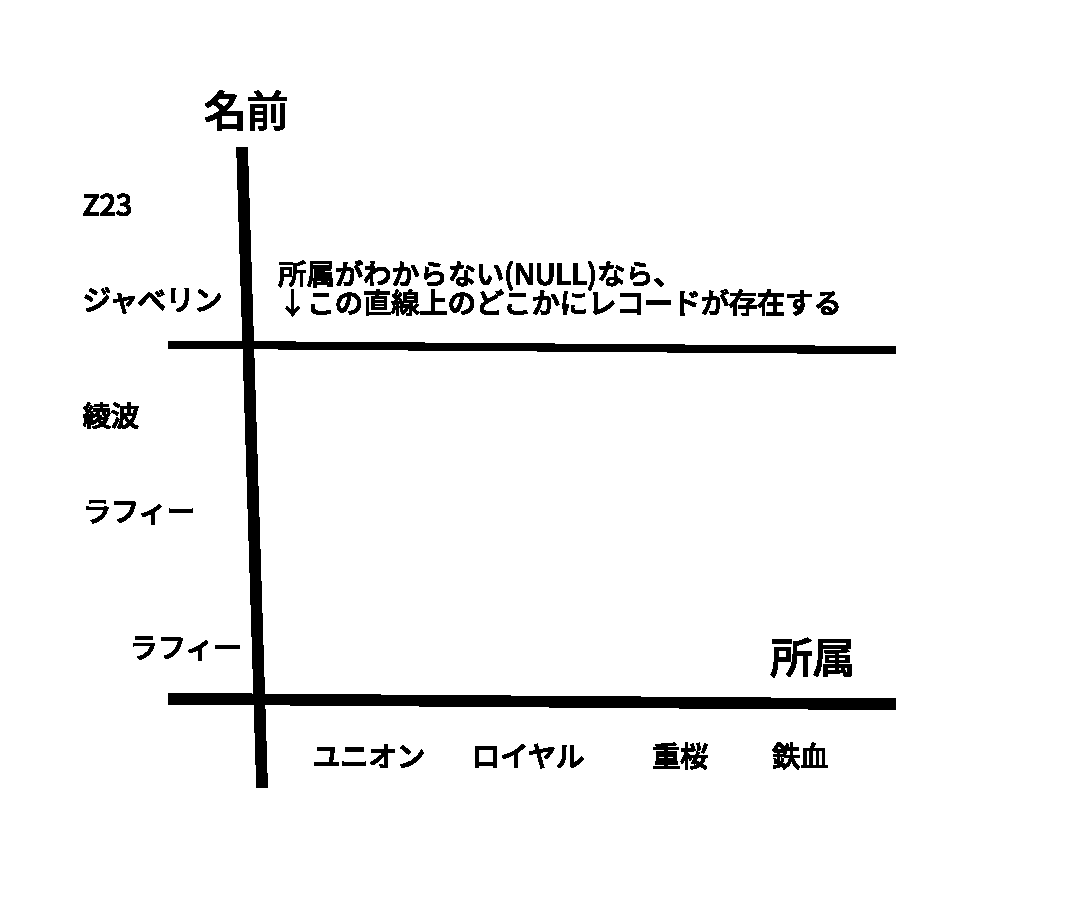
\includegraphics[width=12cm,clip]{draw/unknown.eps}
	\caption{知らないNULLと座標}
	\label{fig:unknown_null}
\end{figure}

知らない、という意味のNULLのときは、ある範囲までしか場所が特定できな、という様に考えることができます。この場合、レコードは、名前の座標軸上の特定の点を通り、所属の座標軸に平行な直線上のどこかにある、というように解釈できます。

\begin{figure}[htbp]
	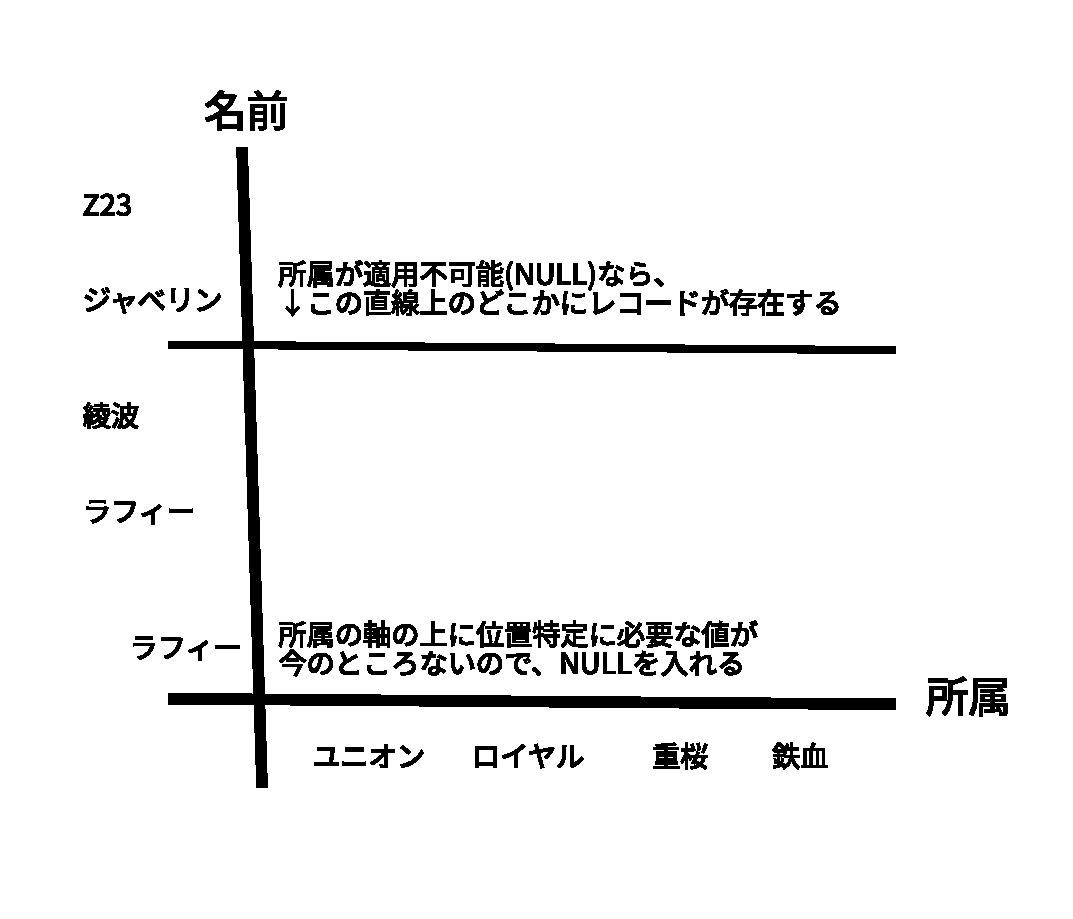
\includegraphics[width=12cm,clip]{draw/not_attach.eps}
	\caption{適用できないNULLと座標}
	\label{fig:not_attach}
\end{figure}

適用できない、というNULLの場合、レコードは、名前の座標上の特定の点を通り、所属の座標軸に平行な直線上のどこかには存在しています。ですが、場所を特定するのに必要な、所属の座標上の値が定義されていない、と解釈します。

テーブルという空間のなかで、レコードが存在している範囲は、どちらの解釈でも同じです。ですが、この範囲内のどこかに存在する、この範囲内のどこにあるか特定するのに必要な値が定義されていない、という文脈上の相違が生じます。これも、文脈的な解釈であって、SQLにはそれを区別するロジックはありません。

\subsection{NULLは使うべきか}

リレーショナルデータベースを説明する文脈でNULLが出てくるとき、多くの場合、NULLには否定的な説明がされます。また、NULLを許容したテーブルにすべきかは、しばしば宗教的な論議を呼びます。そもそもNULLは、あってはならないもなのなのでしょうか。

これは筆者の私見も入りますので、その点はご了承ください。筆者は、必要に応じてNULLは積極的に使っていくべきと考えています。その理由として、NULLとは、それに関しては知らない、という情報をあらわす値であるからです。

また、NULLは、適用できない、という情報を著わす値でもあります。特に、左右の外部結合を行う場合にはさけられないものです。そして、マスタに適用できる情報が無かった、という情報を表す値です。

これらの、知らない、適用できない、という情報を活かすのであれば、NULLは無理に忌避する必要は無いと、筆者は考えています。

その一方、NULLは、情報が無いという情報なのか、情報を入れ忘れているのか、という区別ができないという問題があります。そのため、ロバストネスなシステムを構築する、という観点からは、極力使用すべきではない、という思想もあります。
NULL以外の何らかの値が必須であるアトリビュートについては、NOT NULL属性を付けて、NULLの入力を禁じておくべきでしょう。



\section{NULLと三値論理}

NULLを、知らない、と解釈するとき、これを、真偽がわからないことをあらわす第三の値として用いることができます。つまり、TrueとFalseとUnknownで、真偽と、それが不明であることをあらわします。このとき、NULLは、真か偽か知らない状態、という値として解釈します。

真と偽、という二つの値で論理式を、二値論理と呼んでいます。それに、知らない、という第三の値をくわえたものが三値論理です。では、三値論理の真偽値はどのように考えるのでしょうか。

ここでは、Unknownの概念を論理演算に持ち込んだ、クリーネの強三値論理について説明をします。

\subsection{NULLの考え方}

三値論理では、NULLがあらわす、知らない、という情報をどのように扱うのでしょうか。
NULLは、TrueかFalseかの特定がされていない状態を表します。そして、実際にはTrueとFalseのどちらの可能性もある値として扱われます。

そのため、三値論理の論理演算の結果は、NULLが実際にはどんな値であるか特定されても結果が変化しなければ、TrueかFalseかになります。逆に、特定されることで結果が変わる場合は、結果が分からない、という意味で、NULLとなります。



\subsection{三値論理の記号}

ここでは、三値論理でとりうる値として、TrueとFalsという定数を、真偽をあわらす値として、二値論理から導入します。さらに、NULLがあらわす、知らない、という情報を表す定数として、Unknownを導入します。式では、それぞれ、TとFとUであらわします。

\subsection{NOT演算}

まず、三値論理の論理演算の基本として、否定であるNOT演算をみてみましょう。
Unknownの否定は、Unknowoになります。Knownではありません。なにより、三値論理には、Knownという値はありません。

Unknownは、TrueかFalseかを知らない、という意味です。そのため、Unknownで隠されている値がTrueかFalseか特定されない状態で否定しても、その結果がTrueなのはFalseなのかが決定できません。つまり、Unkonwnの否定を取ってもUnknownになってしまう、ということです。

\begin{table}[htb]
  \begin{tabular}{|c|c|} \hline
    $A$ & $\lnot A$ \\ \hline
    $T$ & $F$ \\
    $F$ & $T$ \\
    $U$ & $U$ \\ \hline
  \end{tabular}
  \label{chart:not}
  \caption{$\lnot A$の真理値表}
\end{table}



\subsection{OR演算}

三値論理のOR演算は、TrueとUnknownの間ではTrueになります。これは、TrueとOR演算をすれば、Unknownが実際にはTrueであってもFalseであってもTrueとなるためです。

また、FalseとUnknownの間では、Unknownになります。これは、UnknownがTrueであればTrue、FalseであればFalseで、結果が変化するためです。

UnknownとUnknownの間のOR演算は、Unknownになります。これは、実際の値がTrueかFalseかが特定できないため、OR演算の結果も特定できないためです。

\begin{table}[htb]
  \begin{tabular}{|c|c|c|} \hline
    $A$ & $B$ & $A \lor B$ \\ \hline
    $T$ & $T$ & $T$ \\
    $T$ & $F$ & $T$ \\
    $T$ & $U$ & $T$ \\
    $F$ & $T$ & $T$ \\
    $F$ & $F$ & $F$ \\
    $F$ & $U$ & $U$ \\
    $U$ & $T$ & $T$ \\
    $U$ & $F$ & $U$ \\
    $U$ & $U$ & $U$\\ \hline
  \end{tabular}
  \label{chart:or}
  \caption{$A \lor B$の真理値表}
\end{table}


\subsection{AND演算}

AND演算は、TrueとUnknownの間ではUnknownになります。これは、UnknownがTrueかFalseかで結果が変化するためです。

また、FalseとUnknownとの間のAND演算は、必ずFalseになります。これは、Unknownの値にかかわらず、FalseとのAND演算の結果は、かならずFalseとなるためです。

UnknownどうしのAND演算は、結果がUnknownとなります。これは、TrueかFalse可が特定できないので、演算の結果を特定できないためです。

\begin{table}[htb]
  \begin{tabular}{|c|c|c|} \hline
    $A$ & $B$ & $A \land B$ \\ \hline
    $T$ & $T$ & $T$ \\
    $T$ & $F$ & $F$ \\
    $T$ & $U$ & $U$ \\
    $F$ & $T$ & $F$ \\
    $F$ & $F$ & $F$ \\
    $F$ & $U$ & $F$ \\
    $U$ & $T$ & $U$ \\
    $U$ & $F$ & $F$ \\
    $U$ & $U$ & $U$\\ \hline
  \end{tabular}
  \label{chart:and}
  \caption{$A \land B$の真理値表}
\end{table}


\subsection{論理包含}

論理包含とは、$A \to B$ と記載します。
AならばBと読み下し、Aという命題と、Bという命題の関係をあらわすものです。
論理包含は、AがTrueのときのみBの真偽を判定する、という言い方もできます。AがFalseであれば、論理包含の結果はTrueとなります。

論理演算の書き方をすると、式\ref{equ:implication}のように書きなおせます。

\begin{equation}
\label{equ:implication}
A \to B = \lnot A \lor B
\end{equation}

たとえば、哺乳類は動物である、という命題をA、パンダは動物である、という命題をBとします。
このとき、哺乳類は動物であるという命題がTrueなので、パンダが動物であるかという命題の結果を、$A \to B$の値とします。
そんため、この例では、$A \to B$がTrueとなります。

もし、Aが哺乳類は植物である、という命題であれば、AはFalseなので、Bの真偽にかかわらず、$A \to B$はTrueとなります。このTrueは、命題AがFalseなので結論が出ない、という意味のTrueです。

\subsubsection{三値論理の論理包含}
三里値論理での倫理包含とは、命題のいずれかがNULLである、つまり、答えが分からない命題があるときに、ならば、という関係に真偽が付けられるのか付けられないのか、ということでもあります。

これまでの、三値論理でのNOTとORから、論理包含の真理値表を作ることができます。

\begin{table}[htb]
  \begin{tabular}{|c|c|c|} \hline
    $A$ & $B$ & $A \to B$ \\ \hline
    $T$ & $T$ & $T$ \\
    $T$ & $F$ & $F$ \\
    $T$ & $U$ & $U$ \\
    $F$ & $T$ & $T$ \\
    $F$ & $F$ & $T$ \\
    $F$ & $U$ & $T$ \\
    $U$ & $T$ & $T$ \\
    $U$ & $F$ & $U$ \\
    $U$ & $U$ & $U$\\ \hline
  \end{tabular}
  \label{chart:impliment}
  \caption{$A \to B$の真理値表}
\end{table}



ここで気をつけるのは、$U \to U$の値はUであるということです。本来、$A \to A$の値はAの値と一致します。これは同語反復と呼ばれる性質です。

Uは、わからない、という意味です。これは、真偽が分からない、という意味であると同時に、そもそもどんな命題なのかが分からない、という解釈をすることができます。そう考えたとき、$\to$の左右のUは、同じ命題なのか違う命題なのか、その判断ができないことになります。

そう考えたとき、$U \to U$の値は、TrueとFalse全ての組み合わせを考慮する必要があり、結果的にUnknownとするのが自然であると考えることができます。
\chapter{UNIONとJOIN}

\section{UNIONすること}

\subsection{UNIONとレコードの重複}

\section{JOINするってどういうこと?}

\subsection{JOINとは可能性を網羅すること}

\subsection{LEFT RIGHT INNER CROSS}


%\chapter{UNIONとJOIN}

\section{UNIONすること}

\subsection{UNIONとレコードの重複}

\section{JOINするってどういうこと?}

\subsection{JOINとは可能性を網羅すること}

\subsection{LEFT RIGHT INNER CROSS}



%\appendix

%\include{adx1}

\backmatter
\begin{thebibliography}{99}
\item
    田中一之 鈴木登志雄
    2003
    『数学のロジックと集合論』
    東京: 培風館
\item
    Celko,J
    ミック 訳
    2013
    『プログラマのためのSQL 第4版』
    東京: 翔泳社
\end{thebibliography}
\chapter{あとがき}

\section*{メイ・カートミル(仮名)とマージ・ニコルス(仮名)の秋葉原での会話}

\begin{quotation}
\noindent
{\bf メイ}「マージさん、なんで私たちの会話があとがきに書いてあるんですか」 \\
{\bf マージ}「読者が見たらメタネタにしか見えないことをぶっこまれても困る」 \\
{\bf メイ}「ところで、この前、スマホの販売員に絡まれたときおとなしかったですね」 \\
{\bf マージ}「次、用途を聞かれたら、カスタムキャストでバ美肉するのに使いますって言ってやろうかな」 \\
\end{quotation}


\section*{後書き}

お兄ちゃん、ADの管理してるのにディレクトリサービスがわからないとか、ADのDはDirectoryの略なの忘れてない?

枕詞のあとですが、まずは、ゆうちゃんさん、今回も表紙をありがとうございます。設定的には、表紙の子は、PostfixとCourier-IMAPによるメールシステム構築(上)の表紙の子の妹、という設定です。

というわけで、インフラエンジニアの毒舌な妹(@infra\_imouto)です.ここ半年は、私に外見がついたり、なんかアドベントカレンダーデビューも果たしたし、自意識までついて仮想筆者になっちゃったり、結構激動でした。

まあそれはおいておいて、このシリーズではある意味いつものことなのですが、資料にできる本が少ないです。特に、ディレクトリの設計に関する本がまったくないというのは問題じゃないかな。
本書でも参考文献にしている「入門LDAP/IpendLDAPディレクトリサービス導入・運用ガイド」の第三版が先日出版されたのですが、どちらかというとLDAPサーバの利用であって、ディレクトリのデザインについては記事がないような。

下巻では、LDAPのデータベースをバックエンドとしたメールシステムの構築をテーマとする予定です。メールシステムは、関連技術が多いため、それを織り込んでいけたらな、と思っています。
Courier-IMAPやCyrus-SASLとの連携、バイナリのビルドなども、そちらで書いていきましょう。

お兄ちゃん、誰がディレクトリの設計とかするんだろうね。みんなそれを忘れていないかな。

\begin{flushright}
2018年12月30日 \\
インフラエンジニアの毒な妹 \\
\end{flushright}

いつもどおりですが、まずは表紙のゆうちゃんさんへの謝辞から。リクエストどおりの子が上がってきて、感謝です。

今回は共著者として、、主に図版を担当した、ありすゆうです。
さて、LDAPのディレクトリ構築について書いた本がなかなかなかったので、本書がその貴重な一冊になれたら、ということを考えながら本書をまとめました。
LDAPはセオリーを覚えてしまえば、それほど難しくはないのですが、そのセオリーを伝える資料というのがなかなか見られません。計算量基準で部分木の配置を決める、というまったく別のノウハウも必要になります。

書き足りない部分として、OIDとPENの説明があります。とはいうものの、これだけでまた本が一冊できそうなテーマなので、どのくらい説明するか難しいところです。OID逆引き辞典という規格もありましたが、流石にページが無茶なことになるのでお蔵入りになりました。

LDAPのデザインについて、少しは残せたのかな、そんなことを考えつつ、ひとまず筆をおくにしましょう。

\begin{flushright}
2018年12月30日 \\
ありす ゆう
\end{flushright}


%\newpage
% ここまでで160ページ鳴ったのでブランクなし
% 1ページブランクを入れる

%\thispagestyle{empty}
%\mbox{}
%\newpage
%\clearpage

% PICOはノンブルがいる
%\thispagestyle{empty}
\mbox{}
\newpage
\clearpage


% PICOはノンブルがいる
%\thispagestyle{empty}

\vspace*{\fill}
\begin{tabular}{ll} \toprule
筆者 & インフラエンジニアの毒舌な妹 ありす ゆう\\
発行 & AliceSystem \\
連絡先 & aliceyou@alicesystem.net \\
URL & http://aliceyou.air-nifty.com/onesan/ \\
初版発行日 & 2018年12月30日 \\
印刷所 & PICO  \\ \bottomrule
\end{tabular}

\end{document}
